\chapter{Theoretical introduction}
	
\section{Problem introduction}
 Theoretical introduction to a problem and mathematical concepts, literature review.... \\
 
\noindent General task is to predict a weather state $\Omega_t$, observed at a timestamp $t$, given $s$ steps from the past, which are essentially previous weather states: $(\Omega_{t-1}, ..., \Omega_{t-s})$. We define $\Omega_t$ as a tensor of a shape: (latitude span, longitude span, features), therefore our complete input data would be 4-dimensional with additional dimension for a time \footnote{To be precise, for neural network based solutions it will be 5-dimensional due to the usage of batches.}. Spatial span was selected so as to cover the border of the whole of Poland and some of its neighbors. More details regarding data are discussed in dataset chapter~\ref{chap:dataset}. High-level spatio-temporal prediction framework is presented at Figure ~\ref{fig:in_out}. \\


\newpage
\subsection{Naming conventions and general prediction framework}
 For further convenience, we propose a general naming convention. 
 \begin{table}[!h]
    \centering
     \begin{tabular}{|c|c|}
        \hline
        Symbol & Description \\
        \hline
        $f_i$ & i-th feature \\
        $s$ & Number of past steps \\
        $fh$ & Forecasting horizon \\
        $\Omega$ & Weather state for all features \\
        $\mathbf{X}$ & $s$-element set of $\Omega$  \\
        $X_t$ & $\Omega$ for timestamp t\\
        $\mathbf{\hat{Y}}$ & $fh$-element set of estimated $\Omega$ \\
        $\hat{Y_t}$ & Estimate of $\Omega$ for timestamp t \\
        $\hat{y_t}^{f_j}$ & Estimate of $\Omega$ for timestamp t and feature $f_j$ \\
        \hline
    \end{tabular}
    \caption{General conventions}
 \end{table}
 
 
%% \noindent We define a $\mathbf{\Phi}$ as a set of baseline models that consist of: 
\begin{table}[!h]
    \centering
    \begin{tabular}{|c|c|}
        \hline
        Model Notation & Model Description \\
        \hline
        $\mathbf{\Phi}_{slr}$ & Simple Linear Regression \\
        $\mathbf{\Phi}_{lr}$  & Linear Regression \\
        $\mathbf{\Phi}_{es}$  & Exponential Smoothing \\
        $\mathbf{\Phi}_{gb}$ & Gradient Boosting Trees \\
        \hline
    \end{tabular}
\caption{Model conventions}
\end{table}
 
%% \noindent Additionally, due to the fact that model $\mathbf{\Phi}_i$ consist of independent models that predicts single feature $f_j$ of a weather state, we can divide it into: 
 
 \noindent Additionally, we define a model $\mathbf{\Phi}_i$ as a set of independent sub-models, where each is responsible only for the prediction of feature $f_j$. This solution was proposed to avoid situations in which ... TODO.
 \[
 \mathbf{\Phi}_{i} = (\Phi_{i}^{f_1}, ..., \Phi_{i}^{f_n})
 \]
 In further considerations, we will use a term sub-models for each of $\Phi_{i}^{f_j}$.


\begin{figure}[!h]



\tikzset{every picture/.style={line width=0.75pt}} %set default line width to 0.75pt        

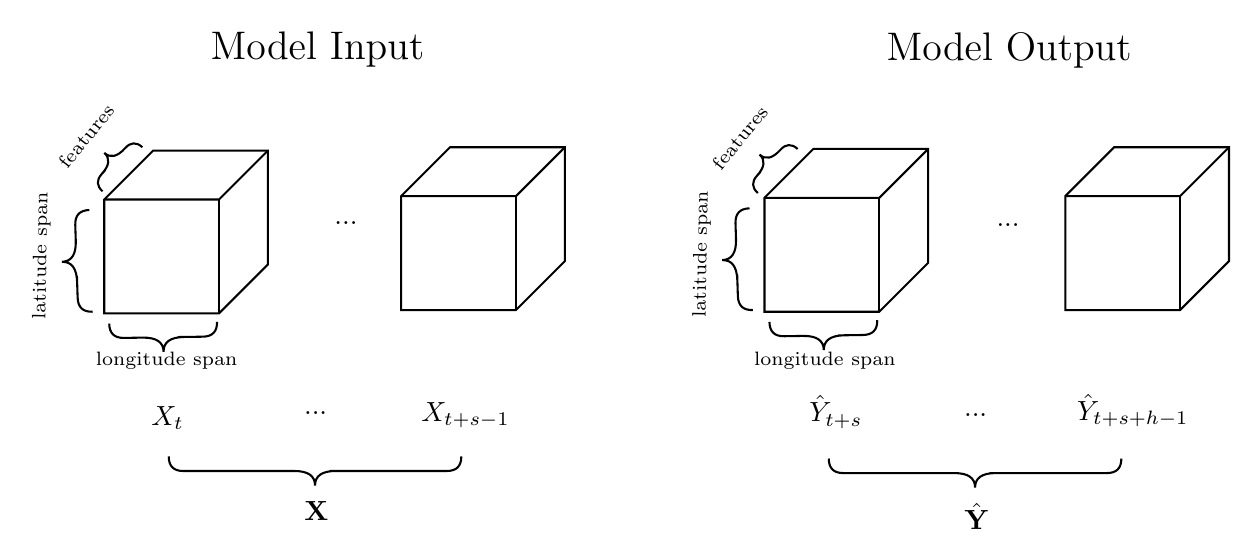
\begin{tikzpicture}[x=0.75pt,y=0.75pt,yscale=-1,xscale=1]
%uncomment if require: \path (0,389); %set diagram left start at 0, and has height of 389

%Shape: Cube [id:dp2816308175879604] 
\draw   (58.25,114.54) -- (81.78,91.01) -- (137.08,91.01) -- (137.08,145.91) -- (113.55,169.44) -- (58.25,169.44) -- cycle ; \draw   (137.08,91.01) -- (113.55,114.54) -- (58.25,114.54) ; \draw   (113.55,114.54) -- (113.55,169.44) ;
%Shape: Brace [id:dp4309828249836092] 
\draw   (76.63,89.37) .. controls (73.72,86.74) and (70.94,86.88) .. (68.31,89.8) -- (68.31,89.8) .. controls (64.55,93.97) and (61.21,94.73) .. (58.29,92.1) .. controls (61.21,94.73) and (60.79,98.13) .. (57.03,102.29)(58.72,100.42) -- (57.03,102.29) .. controls (54.4,105.21) and (54.54,107.99) .. (57.45,110.62) ;
%Shape: Brace [id:dp7756675475750493] 
\draw   (51.06,119.6) .. controls (46.39,119.75) and (44.14,122.16) .. (44.29,126.83) -- (44.53,134.35) .. controls (44.75,141.01) and (42.53,144.42) .. (37.86,144.57) .. controls (42.53,144.42) and (44.97,147.67) .. (45.19,154.34)(45.09,151.34) -- (45.43,161.86) .. controls (45.58,166.52) and (47.99,168.77) .. (52.66,168.62) ;
%Shape: Brace [id:dp612063156099937] 
\draw   (60.65,174.34) .. controls (60.72,179.01) and (63.09,181.3) .. (67.76,181.23) -- (76.73,181.09) .. controls (83.4,180.98) and (86.77,183.26) .. (86.84,187.93) .. controls (86.77,183.26) and (90.06,180.88) .. (96.73,180.78)(93.73,180.82) -- (105.71,180.64) .. controls (110.38,180.57) and (112.67,178.2) .. (112.6,173.53) ;
%Shape: Cube [id:dp42835259632452516] 
\draw   (201.31,112.9) -- (224.84,89.37) -- (280.14,89.37) -- (280.14,144.28) -- (256.61,167.81) -- (201.31,167.81) -- cycle ; \draw   (280.14,89.37) -- (256.61,112.9) -- (201.31,112.9) ; \draw   (256.61,112.9) -- (256.61,167.81) ;
%Shape: Brace [id:dp07592439753840141] 
\draw   (89.33,238.35) .. controls (89.33,243.02) and (91.66,245.35) .. (96.33,245.35) -- (149.81,245.35) .. controls (156.48,245.35) and (159.81,247.68) .. (159.81,252.35) .. controls (159.81,247.68) and (163.14,245.35) .. (169.81,245.35)(166.81,245.35) -- (223.29,245.35) .. controls (227.96,245.35) and (230.29,243.02) .. (230.29,238.35) ;
%Shape: Cube [id:dp7110500253196546] 
\draw   (376.35,113.72) -- (399.88,90.19) -- (455.18,90.19) -- (455.18,145.09) -- (431.65,168.62) -- (376.35,168.62) -- cycle ; \draw   (455.18,90.19) -- (431.65,113.72) -- (376.35,113.72) ; \draw   (431.65,113.72) -- (431.65,168.62) ;
%Shape: Brace [id:dp86120893233015] 
\draw   (392.33,90.19) .. controls (389.42,87.56) and (386.64,87.7) .. (384.01,90.62) -- (384.01,90.62) .. controls (380.25,94.78) and (376.91,95.54) .. (373.99,92.91) .. controls (376.91,95.54) and (376.49,98.94) .. (372.73,103.11)(374.42,101.24) -- (372.73,103.11) .. controls (370.1,106.02) and (370.24,108.8) .. (373.15,111.43) ;
%Shape: Brace [id:dp9673653209625941] 
\draw   (369.15,118.79) .. controls (364.49,118.94) and (362.24,121.34) .. (362.39,126.01) -- (362.63,133.53) .. controls (362.85,140.2) and (360.63,143.6) .. (355.96,143.75) .. controls (360.63,143.6) and (363.07,146.86) .. (363.28,153.52)(363.19,150.52) -- (363.53,161.04) .. controls (363.68,165.71) and (366.09,167.96) .. (370.75,167.81) ;
%Shape: Brace [id:dp9113296386668477] 
\draw   (378.74,173.53) .. controls (378.81,178.2) and (381.18,180.49) .. (385.85,180.42) -- (394.83,180.27) .. controls (401.5,180.17) and (404.87,182.45) .. (404.94,187.12) .. controls (404.87,182.45) and (408.16,180.07) .. (414.83,179.96)(411.83,180.01) -- (423.8,179.82) .. controls (428.47,179.75) and (430.76,177.38) .. (430.69,172.71) ;
%Shape: Cube [id:dp35039842919754816] 
\draw   (521.31,112.9) -- (544.84,89.37) -- (600.14,89.37) -- (600.14,144.28) -- (576.61,167.81) -- (521.31,167.81) -- cycle ; \draw   (600.14,89.37) -- (576.61,112.9) -- (521.31,112.9) ; \draw   (576.61,112.9) -- (576.61,167.81) ;
%Shape: Brace [id:dp3763157845274283] 
\draw   (407.33,239.35) .. controls (407.33,244.02) and (409.66,246.35) .. (414.33,246.35) -- (467.81,246.35) .. controls (474.48,246.35) and (477.81,248.68) .. (477.81,253.35) .. controls (477.81,248.68) and (481.14,246.35) .. (487.81,246.35)(484.81,246.35) -- (541.29,246.35) .. controls (545.96,246.35) and (548.29,244.02) .. (548.29,239.35) ;

% Text Node
\draw (33.24,96.31) node [anchor=north west][inner sep=0.75pt]  [rotate=-309.39,xslant=-0.03] [align=left] {{\scriptsize features}};
% Text Node
\draw (79.43,212.59) node [anchor=north west][inner sep=0.75pt]    {$X_{t}$};
% Text Node
\draw (167.65,123.51) node [anchor=north west][inner sep=0.75pt]   [align=left] {...};
% Text Node
\draw (21.86,173.65) node [anchor=north west][inner sep=0.75pt]  [rotate=-270.99] [align=left] {{\scriptsize latitude span}};
% Text Node
\draw (52.73,186.5) node [anchor=north west][inner sep=0.75pt]   [align=left] {{\scriptsize longitude span}};
% Text Node
\draw (209.49,210.96) node [anchor=north west][inner sep=0.75pt]    {$X_{t+s-1}$};
% Text Node
\draw (153.04,215.29) node [anchor=north west][inner sep=0.75pt]   [align=left] {...};
% Text Node
\draw (153.16,258.53) node [anchor=north west][inner sep=0.75pt]    {$\mathbf{X}$};
% Text Node
\draw (433.72,32.89) node [anchor=north west][inner sep=0.75pt]   [align=left] {{\Large Model Output}};
% Text Node
\draw (108.05,32.26) node [anchor=north west][inner sep=0.75pt]   [align=left] {{\Large Model Input}};
% Text Node
\draw (348.14,97.12) node [anchor=north west][inner sep=0.75pt]  [rotate=-309.39,xslant=-0.03] [align=left] {{\scriptsize features}};
% Text Node
\draw (339.95,172.84) node [anchor=north west][inner sep=0.75pt]  [rotate=-270.99] [align=left] {{\scriptsize latitude span}};
% Text Node
\draw (369.83,186.68) node [anchor=north west][inner sep=0.75pt]   [align=left] {{\scriptsize longitude span}};
% Text Node
\draw (486.65,124.51) node [anchor=north west][inner sep=0.75pt]   [align=left] {...};
% Text Node
\draw (396.43,207.59) node [anchor=north west][inner sep=0.75pt]    {$\hat{Y}_{t+s}$};
% Text Node
\draw (525.49,206.96) node [anchor=north west][inner sep=0.75pt]    {$\hat{Y}_{t+s+h-1}$};
% Text Node
\draw (471.04,216.29) node [anchor=north west][inner sep=0.75pt]   [align=left] {...};
% Text Node
\draw (471.16,259.53) node [anchor=north west][inner sep=0.75pt]    {$\hat{\mathbf{Y}}$};


\end{tikzpicture}


\caption{Spatio-Temporal prediction framework}  \label{fig:in_out} 


\end{figure}


\noindent Take into account the fact that this framework may differ when applying techniques such as grid neighbors~\ref{chap:neighbors} or using constants encodings~\ref{chap:feat_eng}. Details regarding those differences are explained deeply in subsequent chapters.

 \newpage
 
 \subsection{Literature review}
 After stating the problem we want to shortly inspect current research and results in this field... \\
Short review of quality papers related to this problem; explanation of what was already achieved in this task - SOTA solutions, especially emphasizing GraphCast paper; what we want to reproduce or compare ourself with. \\
\noindent Maybe start with: ~\cite{WFConsiderations}

\section{Explored techniques}
 \subsection{Autoregression}
 \noindent Each baseline model is designed to predict the entire weather state for only the next timestamp - unit forecasting horizon. Therefore, when applying our models for short-term prediction task of a few timestamps into the future, the autoregressive approach is commonsensical. \\ \\
 
 \noindent Let's define model input as $\mathbf{X}$, a vector of $s$ weather states: 
 \[
 \mathbf{X} = (X_{t}, ..., X_{t+s-1})
 \]
 and output of a model as $\mathbf{\hat{Y}}$, which consist of $fh$ forecasted states:
 \[
 \mathbf{\hat{Y}} = (\hat{Y}_{t+s}, ..., \hat{Y}_{t+s+fh-1})
 \]
 
 \noindent Autoregressive prediction is $fh$-steps process such that:
 \begin{flalign*}
    &\hat{Y}_{t+s} = \mathbf{\Phi}_{i}(X_{t}, ..., X_{t+s-1}) \\
    &\hat{Y}_{t+s+1} = \mathbf{\Phi}_{i}(X_{t+1}, ..., X_{t+s-1}, \hat{Y}_{t+s}) \\
    &\vdots \\
    &\hat{Y}_{t+s+fh-1} = \mathbf{\Phi}_{i}(X_{t+fh-1}, ...,  \hat{Y}_{t+s+fh-3}, \hat{Y}_{t+s+fh-2})
 \end{flalign*}

 \noindent Therefore, oversimplifying:
 \[
    \mathbf{\hat{Y}} = \mathbf{\Phi_{i}(X)}
 \]
 
 \noindent For each model except $\mathbf{\Phi}_{slr}$, during every autoregressive step concatenation of outputs from sub-models is required, whereas $X_t$ needs to have information from every feature:
 \begin{flalign*}
    &\hat{y}_t^{f_j} = \Phi_{i}^{f_j}(\mathbf{X}) \\
    &\hat{Y}_{t} = (\hat{y}_t^{f_0}, ..., \hat{y}_t^{f_n}) \\
 \end{flalign*}
 
\newpage
\subsection{Grid Neighbors}\label{chap:neighbors}

\noindent For each input tensor we've implemented though called additional neighbors technique. It is expanding each of our data points to store information about closely located grid boxes. They're chosen based on the relative distance (radius) between the center of grid-boxes: $r$. On underneath figure, grid boxes colored grey represents relative data point and black boxes are its neighbors.

\begin{figure}[!ht]
    \centering
    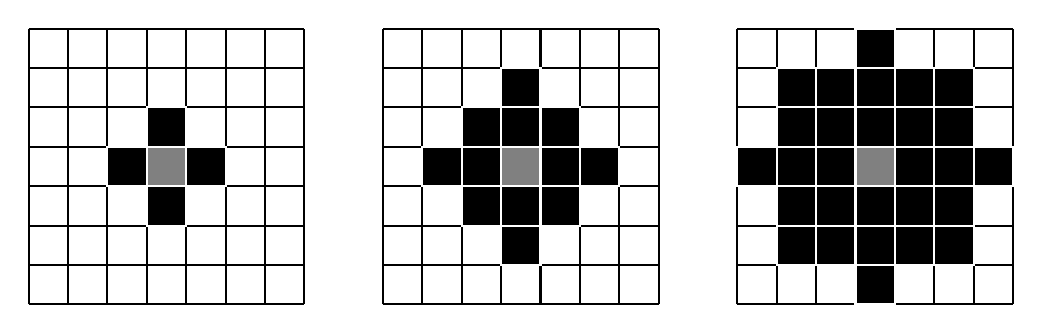
\begin{tikzpicture}[scale=0.5]
        \draw[step=1, black] (0,0) grid (7,7);
        \filldraw[fill=gray, draw=white] (3,3) rectangle (4,4);
        \filldraw[fill=black, draw=white] (3,2) rectangle (4,3);
        \filldraw[fill=black, draw=white] (2,3) rectangle (3,4);
        \filldraw[fill=black, draw=white] (3,4) rectangle (4,5);
        \filldraw[fill=black, draw=white] (4,3) rectangle (5,4);
        
        \begin{scope}[shift={(9,0)}]
            \draw[step=1, black] (0,0) grid (7,7);
            \foreach \i in {1, ..., 9} {
                \pgfmathtruncatemacro\row{mod(\i-1,3)}
                \pgfmathtruncatemacro\col{int((\i-1)/3)}
                \filldraw[fill=black, draw=white] (\row+2,\col+2) rectangle (\row+3,\col+3);
            }
            \filldraw[fill=gray, draw=white] (3,3) rectangle (4,4);
            \filldraw[fill=black, draw=white] (1,3) rectangle (2,4);
            \filldraw[fill=black, draw=white] (5,3) rectangle (6,4);
            \filldraw[fill=black, draw=white] (3,1) rectangle (4,2);
            \filldraw[fill=black, draw=white] (3,5) rectangle (4,6);
        \end{scope}

        \begin{scope}[shift={(18,0)}]
            \draw[step=1, black] (0,0) grid (7,7);
            \foreach \i in {1, ..., 25} {
                \pgfmathtruncatemacro\row{mod(\i-1,5)}
                \pgfmathtruncatemacro\col{int((\i-1)/5)}
                \filldraw[fill=black, draw=white] (\row+1,\col+1) rectangle (\row+2,\col+2);
            }
            \filldraw[fill=gray, draw=white] (3,3) rectangle (4,4); 
            \filldraw[fill=black, draw=white] (0,3) rectangle (1,4);
            \filldraw[fill=black, draw=white] (6,3) rectangle (7,4);
            \filldraw[fill=black, draw=white] (3,0) rectangle (4,1);
            \filldraw[fill=black, draw=white] (3,6) rectangle (4,7);
        \end{scope}
    \end{tikzpicture}
    \caption{Neighbors logic for $r=(1,2,3)$}
    \label{fig:neighbors}
\end{figure}

%Formal definition of a neighbors set $N$ for all of grid boxes $v$, where $V$ is a set of all:
\noindent Formal definition, assuming that grid boxes has resolution (1x1):
\begin{table}[!h]
    \centering
    \begin{tabular}{|c|c|}
        \hline
        Symbol & Description \\
        \hline
        $v_{i,j}$ & Grid box at latitude $i$ and longitude $j$ \\
        $V$  & Set of all grid boxes \\
        $\|v_{m,n} - v_{i,j}\|^2$  & Euclidian distance between centres of $v_1$ and $v_2$ \\
        $N_v$ & Set of neighbors for grid box $v$ \\
        \hline
    \end{tabular}
\end{table}
\[
    \forall v_{i,j} \in V: \{\forall v_{m,n \neq i,j} : \|v_{m,n} - v_{i,j}\|^2 \le r\} \in N_{v_{i,j}}
\]

\noindent Unfortunately, the trade-off between memory footprint, computational complexity, and performance gain was not sufficient to incorporate and test bigger $r$ values.

 
 \section{Baselines}
 \subsection{Exponential Smoothing}
 \subsection{Simple Linear Regression}
 \subsection{Linear Regression}
 
 \[
    \mathbf{X} \boldsymbol\beta = \mathbf{\hat{Y}}
 \]
 
 \[
    \begin{bmatrix}
    x_{11} & x_{12} & \cdots & x_{1n}\\
    x_{21} & x_{22} & \cdots & x_{2n}\\
    \vdots & \vdots & \ddots & \vdots\\
    x_{n1} & x_{n2} & \cdots & x_{nn}
    \end{bmatrix}
    \begin{bmatrix}
    \beta_1\\\beta_2\\ \vdots\\b_n
    \end{bmatrix}
    =\begin{bmatrix}
    \hat{y_1}\\\hat{y_2}\\ \vdots\\\hat{y_n}
    \end{bmatrix}
\]
 \subsection{Gradient Boosting}
 \subsection{UNet}


\section{Neural network concept}
Optional? \\

\noindent Explain architecture of dense neural networks and other types such as convolutional, recurrent, graph (depending on which one eventually will be used).

\section{GraphCast}
Deep dive into GraphCast architecture.

\section{Model}
Proposed model architecture and comparision with GraphCast. \\

\noindent After briefly testing multiple Graph Convolutional Cells that support edge feature vectors, we have concluded that the most promising results and sufficient computation time are obtained by TransformerConv ~\cite{shi2021masked}.\\

\noindent Multi-layer perceptron as an embedder converting features dimension into more abstract latent space that stores better representation of weather state.

.... \\

\noindent Multi-layer perceptron as a decoder converting encoded features into its natural representation.


\begin{flalign*}
    X = MLP^{Embedder}(X) \\
    X = GNN_1(X) \\
    ...         \\
    X = GNN_N(X) \\
    \hat{Y} = MLP^{Decoder}(X) \\
 \end{flalign*}

\subsection{Additional techniques and feature engineering}\label{chap:feat_eng}
Present concept of spatial-mapping, edge attributes. Explain spatial and temporal feature encodings as well as usage of constants like geopotential. 

\begin{flalign*}
    d_{V_i,V_j} &= \sqrt{(V_{j_x} - V_{i_x})^2 + (V_{j_y} - V_{i_y})^2} \\
    e_{V_i,V_j} &= (V_{j_x} - V_{i_x}, V_{j_y} - V_{i_y}, d_{V_i,V_j})
\end{flalign*}
 
